%
% File acl2014.tex
%
% Contact: giovanni.colavizza@epfl.ch
%%
%% Based on the style files for ACL-2013, which were, in turn,
%% Based on the style files for ACL-2012, which were, in turn,
%% based on the style files for ACL-2011, which were, in turn, 
%% based on the style files for ACL-2010, which were, in turn, 
%% based on the style files for ACL-IJCNLP-2009, which were, in turn,
%% based on the style files for EACL-2009 and IJCNLP-2008...

%% Based on the style files for EACL 2006 by 
%%e.agirre@ehu.es or Sergi.Balari@uab.es
%% and that of ACL 08 by Joakim Nivre and Noah Smith

\documentclass[11pt]{article}
\usepackage{acl2014}
\usepackage{times}
\usepackage{url}
\usepackage{latexsym}
\usepackage{graphicx}	% For figure environment
\usepackage{hyperref}


%\setlength\titlebox{5cm}

% You can expand the titlebox if you need extra space
% to show all the authors. Please do not make the titlebox
% smaller than 5cm (the original size); we will check this
% in the camera-ready version and ask you to change it back.


\title{Event detection on a Twitter dataset}

\author{ 
  Albrici Tanguy \hspace{40px} \\
  {\tt tanguy.albrici@epfl.ch} \hspace{40px} \And
  Di Dio Davide \\
  {\tt davide.didio@epfl.ch} \And
   \hspace{40px} Bruno Wicht \\
{\tt \hspace{40px} bruno.wicht@epfl.ch} \\}

\date{}

\begin{document}
\maketitle
\begin{abstract}
  Social networks now have a huge importance in our lives and many people use them to comment about events that are happening around the globe. With this project, we would like to see how the Swiss Twitter community reacts to important events happening in Switzerland or around the world. Our main goal is to determine to what extent and how well we can learn about what is happening in the world or in our country based on the Swiss tweets. The story we want to tell is the evolution of tweets during important events between 2010 and 2016 and discover what kind of events Swiss people are tweeting about the most. We are motivated to do this project and tell this story because none of us are active on Twitter and we're interested in understanding better how twitter is used in Switzerland.
\end{abstract}

\section{Credits}


\section{Introduction}


\section{Pre-processing}

At first, we extract the hashtags from each tweets. Each tweet is stored in a dataframe that only contains the informations we require, namely: 
\begin{itemize}

\item The tweet id 
\item The user id
\item The longitude and latitude
\item The hashtags extracted from the text
\item The day, month and year of the tweet creation

\end{itemize}

After the hashtag extraction, we only keep the tweets with at least one hashtag.


\section{Data Manipulation}


\subsection{Grouping by hashtag}

In order to implement event detection efficiently, we need to compute a dictionary containing for each hashtags the ids of each post that contains it. This is done in the function \texttt{group\_by\_hashtag(...)}. This function iterates over every post in the database and adds the id of the post in the dictionary entry of the hashtag. In this method, we also compute the number of unique authors for this hashtag. With this value, we can easily filter out hashtags if they only concern few posters.


\section{Data analysis and visualization}

This section covers how we visualize our data and allow us to get a feel on how to detect events.

\subsection{Visualizing hashtag frequency}

\begin{figure}[htbp]
  \vspace*{-1mm}
  \centering
  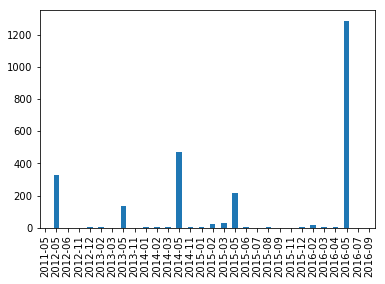
\includegraphics[width=\columnwidth]{figures/freq_month_eurovision.png}
  \vspace{-5mm}
  \caption{For the top months, plot the number of tweets with  \texttt{\#eurovision}}
  \label{fig:freq_month_eurovision}
\end{figure}

With frequency visualisation, we can visualize spikes in the number of tweets. The method \texttt{plot\_frequency\_tags(...)} computes for a given hashtag the numbers of tweets per frequency that contain this hashtag. Here we can chose frequency as either day, month or year. Then it takes the \texttt{n} most tweeted dates and displays them in chronological order with a bar plot. We only take the \texttt{n} most tweeted dates because it provides the most compact visualisation. Note however that these plot are not homogenous in time. 

Now, let us look a the frequency plot \ref{fig:freq_month_eurovision} for \texttt{\#eurovision} .
We can very clearly see an increase in the number of tweet during the month of may of each years. Since eurovision takes place in may, it is obvious that people will more likely talk about it during it's happening. We will be using this knowledge to develop an algorithm to detect those sudden spikes.

\subsection{Visualizing event localisation}

\begin{figure}[htbp]
  \vspace*{-1mm}
  \centering
  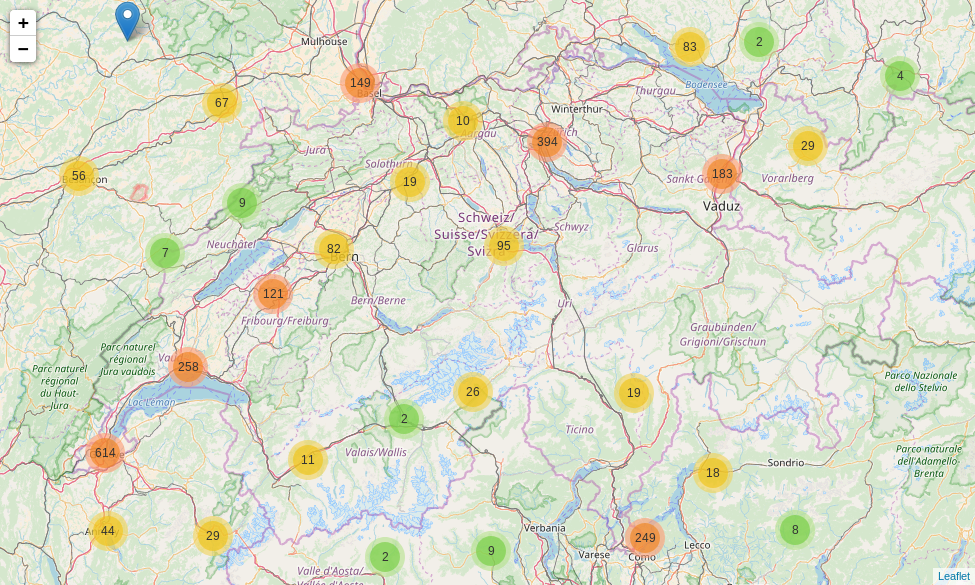
\includegraphics[width=\columnwidth]{figures/map_eurovision.png}
  \vspace{-5mm}
  \caption{Map with every tweet for \texttt{\#eurovision}}
  \label{fig:map:eurovision}
\end{figure}

\begin{figure}[htbp]
  \vspace*{-1mm}
  \centering
  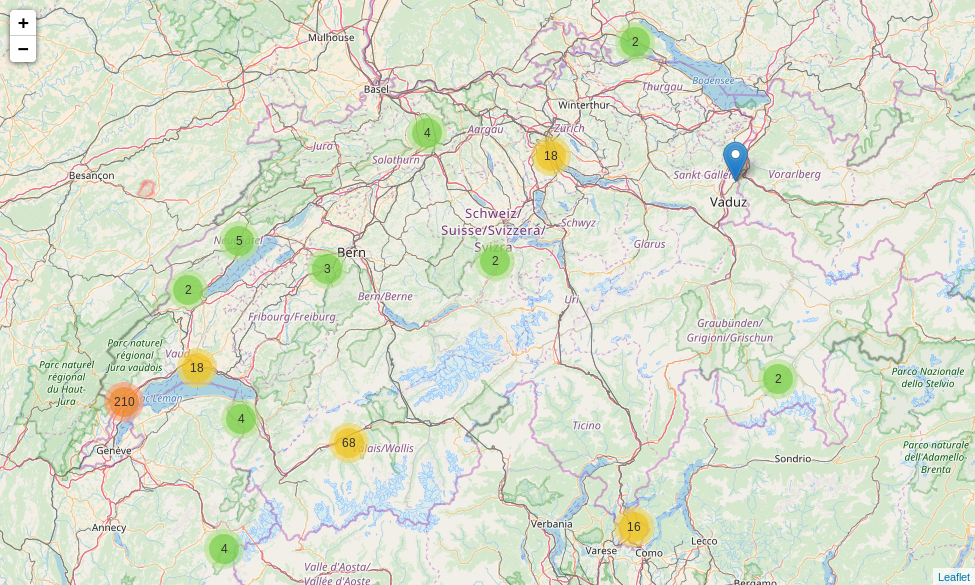
\includegraphics[width=\columnwidth]{figures/map_paleo.png}
  \vspace{-5mm}
  \caption{Map with every tweet for \texttt{\#paleo}}
  \label{fig:map_paleo}
\end{figure}

The map are displayed in order to get an intuition on the geographic repartitions of tweets. The map are created using folium. We use a MarkerCluster to group every tweet close in space. Other than that, it is a pretty straight forward folium map. Now, look at the first map\ref{fig:freq_day_paleo}. We see that the distribution is regrouped in the cities but overall it is quite uniform if we consider the population density. On the other side, in the second map \ref{fig:map_paleo}, we see that most of the tweets are located in Nyon (this is where the festival takes place). The logic here is that only people close to the event are aware of its happening and will more likely talk about it. Whereas international event are known in switzerland as a whole. Hence a local events lead to tweet localisation around the position of the event and international events have a spread tweet geographic distribution. We will use this knowledge to find the type of an event.


\section{Event detection}


\begin{thebibliography}{}

\bibitem[\protect\citename{Gusfield}1997]{Gusfield:97}
Dan Gusfield.
\newblock 1997.
\newblock {\em Algorithms on Strings, Trees and Sequences}.
\newblock Cambridge University Press, Cambridge, UK.

\end{thebibliography}

\end{document}
